\documentclass[tikz]{standalone}

\usepackage{tikz}
\usepackage{amsmath, amssymb}

\usetikzlibrary{shapes.geometric, positioning, calc, fit}
\tikzstyle{block} = [draw, fill=white, minimum width=1.5cm, 
        minimum height=0.7cm]
\tikzstyle{expand} = [draw, fill=white, trapezium, trapezium angle=60,
        minimum width=2.5cm]
\tikzset{XOR/.style={draw,circle,append after command={
    [shorten >=\pgflinewidth, shorten <=\pgflinewidth,]
    (\tikzlastnode.north) edge (\tikzlastnode.south)
    (\tikzlastnode.east) edge (\tikzlastnode.west)
        }
    }
}
\begin{document}
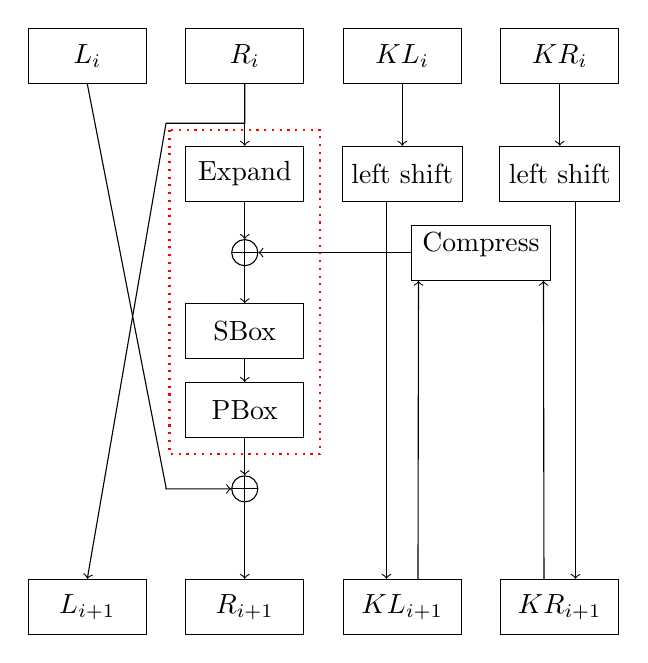
\begin{tikzpicture}
    \node [block] (Li) {$L_i$};
    \node [block, right of=Li, node distance=2cm] (Ri) {$R_i$};
    \node [block, below of=Ri, node distance=1.5cm] (Ei) {Expand};
    \node [XOR, below of=Ei, node distance=1cm] (xi) {};
    \node [block, below of=xi, node distance=1cm] (Si) {SBox};
    \node [block, below of=Si, node distance=1cm] (Pi) {PBox};
    \node [XOR, below of=Pi, node distance=1cm] (xj) {};
    \node [block, below of=xj, node distance=1.5cm] (Rj) {$R_{i+1}$};
    \node [block, left of=Rj, node distance=2cm] (Lj) {$L_{i+1}$};

    \node [block, right of=Ri, node distance=2cm] (KLi) {$KL_i$};
    \node [block, right of=KLi, node distance=2cm] (KRi) {$KR_i$};
    \node [block, below of=KLi, node distance=1.5cm] (li) {left shift};
    \node [block, right of=li, node distance=2cm] (ri) {left shift};
    \node [block, fit={($(li.west)+(1,0)$) ($(ri.east)+(-1,0)$)}, yshift=-1cm] (compress) {Compress};
    \node [block, right of=Rj, node distance=2cm] (KLj) {${KL_{i+1}}$};
    \node [block, right of=KLj, node distance=2cm] (KRj) {${KR_{i+1}}$};

    \draw[->] (Ri) -- (Ei);
    \draw[->] (Ei) -- (xi);
    \draw[->] (xi) -- (Si);
    \draw[->] (Si) -- (Pi);
    \draw[->] (Pi) -- (xj);
    \draw[->] (xj) -- (Rj);
    \draw[->] (Ri.south) -- ++(0,-0.5) -- ++(-1,0) -- (Lj.north);
    \draw[->] (Li.south) -- ++(1,-5.125) |- (xj.west);
    \draw[red,thick,dotted] ($(Ei.north west)+(-0.2,0.2)$) 
        rectangle ($(Pi.south east)+(0.2,-0.2)$);
    
    \draw[->] (KLi) -- (li);
    \draw[->] (KRi) -- (ri);
    \draw[->] ($(li.south)+(-0.2,0)$) -- ($(KLj.north)+(-0.2,0)$); 
    \draw[->] ($(ri.south)+(+0.2,0)$) -- ($(KRj.north)+(+0.2,0)$);

    \draw[->] ($(KLj.north)+(+0.2,0)$) -- ($(compress.south west)+(+0.1,0)$);
    \draw[->] ($(KRj.north)+(-0.2,0)$) -- ($(compress.south east)+(-0.1,0)$);

    \draw[->] (compress.west) -- (xi.east);
\end{tikzpicture}
\end{document}